\chapter{基于随机排列的高效大语言模型推理框架}
大语言模型(Large Language Models,简称大模型)的出现给隐私保护机器学习带来了新的挑战。
%
一方面,由于大模型的参数量和计算量庞大,基于密码学的隐私推断方法面临着极为严重的性能问题;另一方面,由于大模型的结构影响,拆分学习等暴露中间结果的方法无法保证隐私。
%
为了实现更为高效和安全的大模型隐私推断,本章在第\ref{chap:ss-perm}章的基础上,优化秘密分享的乘法协议和基于随机排列的非线性函数协议,同时采用同态加密实现预测层,实现了高效的大模型隐私推断框架PermLLM。
%
PermLLM框架能够在现实网络环境下实现秒级别的大模型隐私推断,比已有的基于密码学的方案提升了超过两个数量级。

\section{研究背景}
2023年ChatGPT的出现,标志着人工智能的发展到达了一个新的阶段~\cite{chatgpt}。
%
ChatGPT以及类似的大语言模型(Large Language Models),通过利用大量的语料进行自回归训练以及人类反馈强化学习,从而实现了与人类进行自然对话的能力,并且在大量任务上都达到了最先进水平~\cite{}。
%
通过提示词,大模型可以完成多种多样的任务,其效果往往超过此前研究者针对该任务精心设计的模型~\cite{}。
%
因此,当前大语言模型成为了学术界和业界的焦点,基于大语言模型的应用也层出不穷,包括了各种领域的问题回答(Question Answering)、阅读理解(Reading Comprehension)、文本生成(Text Generation)、检索增强(Retrieval Augmented Generation)等~\cite{}。


在大模型被广泛应用的同时,其隐私问题也愈加突出。
%
大模型的训练成本极大,据估计,一个GPT-3模型训练的计算成本已经高达数百万美金。
%
因此,大模型的模型参数是公司的重要资产,不能直接以开源的方式提供给用户。
%
在这种情况下,用户必须调用模型拥有方(如OpenAI公司)提供的接口(API)来使用大模型。
%
用户将自身的输入文本发送给模型拥有方的服务器,服务器上执行明文的大模型推断,然后将结果返还给用户。
%
在这个过程中,用户输入文本的隐私就被完全暴露给了模型拥有方。
%
这带来了极大的隐私泄漏风险。
%
例如,三星公司的员工使用ChatGPT分析了公司内部的机密数据,使得三星公司开始禁止员工使用类似的大模型工具~\cite{}。
%
因此,上述的隐私泄露风险给大语言模型的应用产生了一定程度的阻碍。


为了解决大模型的隐私问题,在应用大模型时同时保护用户输入和模型参数的隐私,一些研究基于密码学方法提出了初步的解决方案。
%
这些方法一般采用已有的秘密分享或同态加密方案来实现大模型中的线性运算,然后采用高阶多项式拟合的方式来实现大模型中的非线性运算,如GeLU、Softmax等。
%
但是由于采用密码学的隐私保护机器学习框架自身会带来巨大的额外开销,加之大模型的参数规模和运算量十分庞大,上述方法即使在理想的计算资源与网络环境下,也至少需要消耗几分钟时间、数十GB流量才能产生一个输出单词。
%
因此,基于密码学方法的大模型隐私推断框架的实用性依然欠缺,并且可以预见到使用已有的密码学底层算法很难实现具备实用性的大模型隐私推断。
%
如何在保护输入的模型隐私的基础上,实现高效安全的实现大模型推断,依然是一个亟待解决的问题。

\section{初步研究}
本节我们对大语言模型的模型结构进行初步的介绍和分析,并从理论和实验两方面分析使用拆分学习进行大模型隐私推断时的严重隐私泄漏问题。

\subsection{大模型结构}
当前的大语言模型都是基于Transformer架构~\cite{vaswani_2017_attention}实现的,其模型可以分为3层,分别是:
\begin{enumerate}
    \item 输入词向量(Word Embedding):即一个嵌入向量矩阵$E \in \mathbb R^{n\times d}$,其中$n$表示词汇表大小,$d$表示词向量的维度,一般为4096。
    %
    当输入$n$个单词(Token)后,其输出为$n \times d$大小的矩阵。
    %
    \item Transformer层:包含了多层Transformer结构,对隐层表征进行多次变换,其输入和输出的矩阵大小均为$n \times d$(此处忽略批样本情况,进考虑三个样本)。
    \item 输出词向量:与输入词向量相同,包含了一个矩阵$E' \in \mathbb R^{n\times d}$,且一般来说$E' = E$。
    当获得Transformer层的输出后,对输出的最后一行计算分数$\bvec  s = E'\bvec h$,表示输出单词的概率分布。
\end{enumerate}

其中Transformer层的关键模块是多头自注意力机制(Multi-Head Self-Attention,简称MHA)。
%
该模块会融合文本中不同位置单词(上下文)的信息产生输出,而其他模块仅仅对当前位置的表征进行变换。
%
具体而言,对于隐层表征$H \in \mathbb R^{n\times d}$,多头自注意力机制的运算包含如下步骤:
\begin{enumerate}
    \item 产生查询(Query)、键(Key)、值(Value)对应的向量:对于任意一个位置的隐层表征$\bvec h \in H$,通过线性投影产生对应的$\bvec q = W_q \bvec h, \bvec k = W_k \bvec h, \bvec v = W_v \bvec h \in \mathbb R^d$。
    %
    \item 将所有的查询、键、值向量分割为维度为$d'$的子向量(注意力头),总共$d/d'$个,并对其进行位置嵌入(Positional Embedding)变换,一般而言是对向量逐元素地加或乘一个固定并和当前单词相关的向量。
    %
    \item (对于每个注意力头)对于第$i$个查询$\bvec q_i'$,将其与当前存在的所有的键作内积得到分数$s'_{i, j} = \bvec q_i' \cdot \bvec k_j, j = 1\cdots n$。
    对这些分数进行Softmax归一化后再计算加权的值向量和 $\bvec h'_i = \dfrac{\exp {s'_{i, j}}}{\sum_{k = 1}^n \exp {s'_{i, k}}} \cdot \bvec v_j \in \mathbb R^{d'}$,这是当前的注意力头的输出。
    %
    \item 将各个注意力头的输出拼接起来,得到多头注意力的输出$\bvec h_i = \mathsf{concat}(\cdots, \bvec h'_i, \cdots)$。
\end{enumerate}

从上述分析中可以看出,注意力机制将不同位置(也就是不同输入单词)对应的表征进行了相互融合,从而捕捉文本中上下文的关系。
%
大语言模型在生成文本时,需要采用迭代生成的方式,即将前一轮的输出单词拼接到当前的输入语句中,然后再次输入模型预测下一个单词。
%
由于我们仅仅需要最后一个单词对应的表征,我们可以把之前MHA中计算出来的键向量和值向量缓存下来,从而只需要把最后一个单词输入模型中即可计算,从而避免重复计算。
%
这种技术被称为键值缓存(KV Cache)~\cite{pope_2023_efficiently_kv_cache}。
%
Transformer的其他模块包括全连接层(Fully-Connect Layer)、层归一化(Layer Normalization)模块,以及残差连接,是普通神经网络中的常用模块,在此不再赘述。
%
\autoref{fig:perm-llm_llm-arch}展现了一个典型的大语言模型的网络结构。

\begin{figure}[htbp]
    \centering
    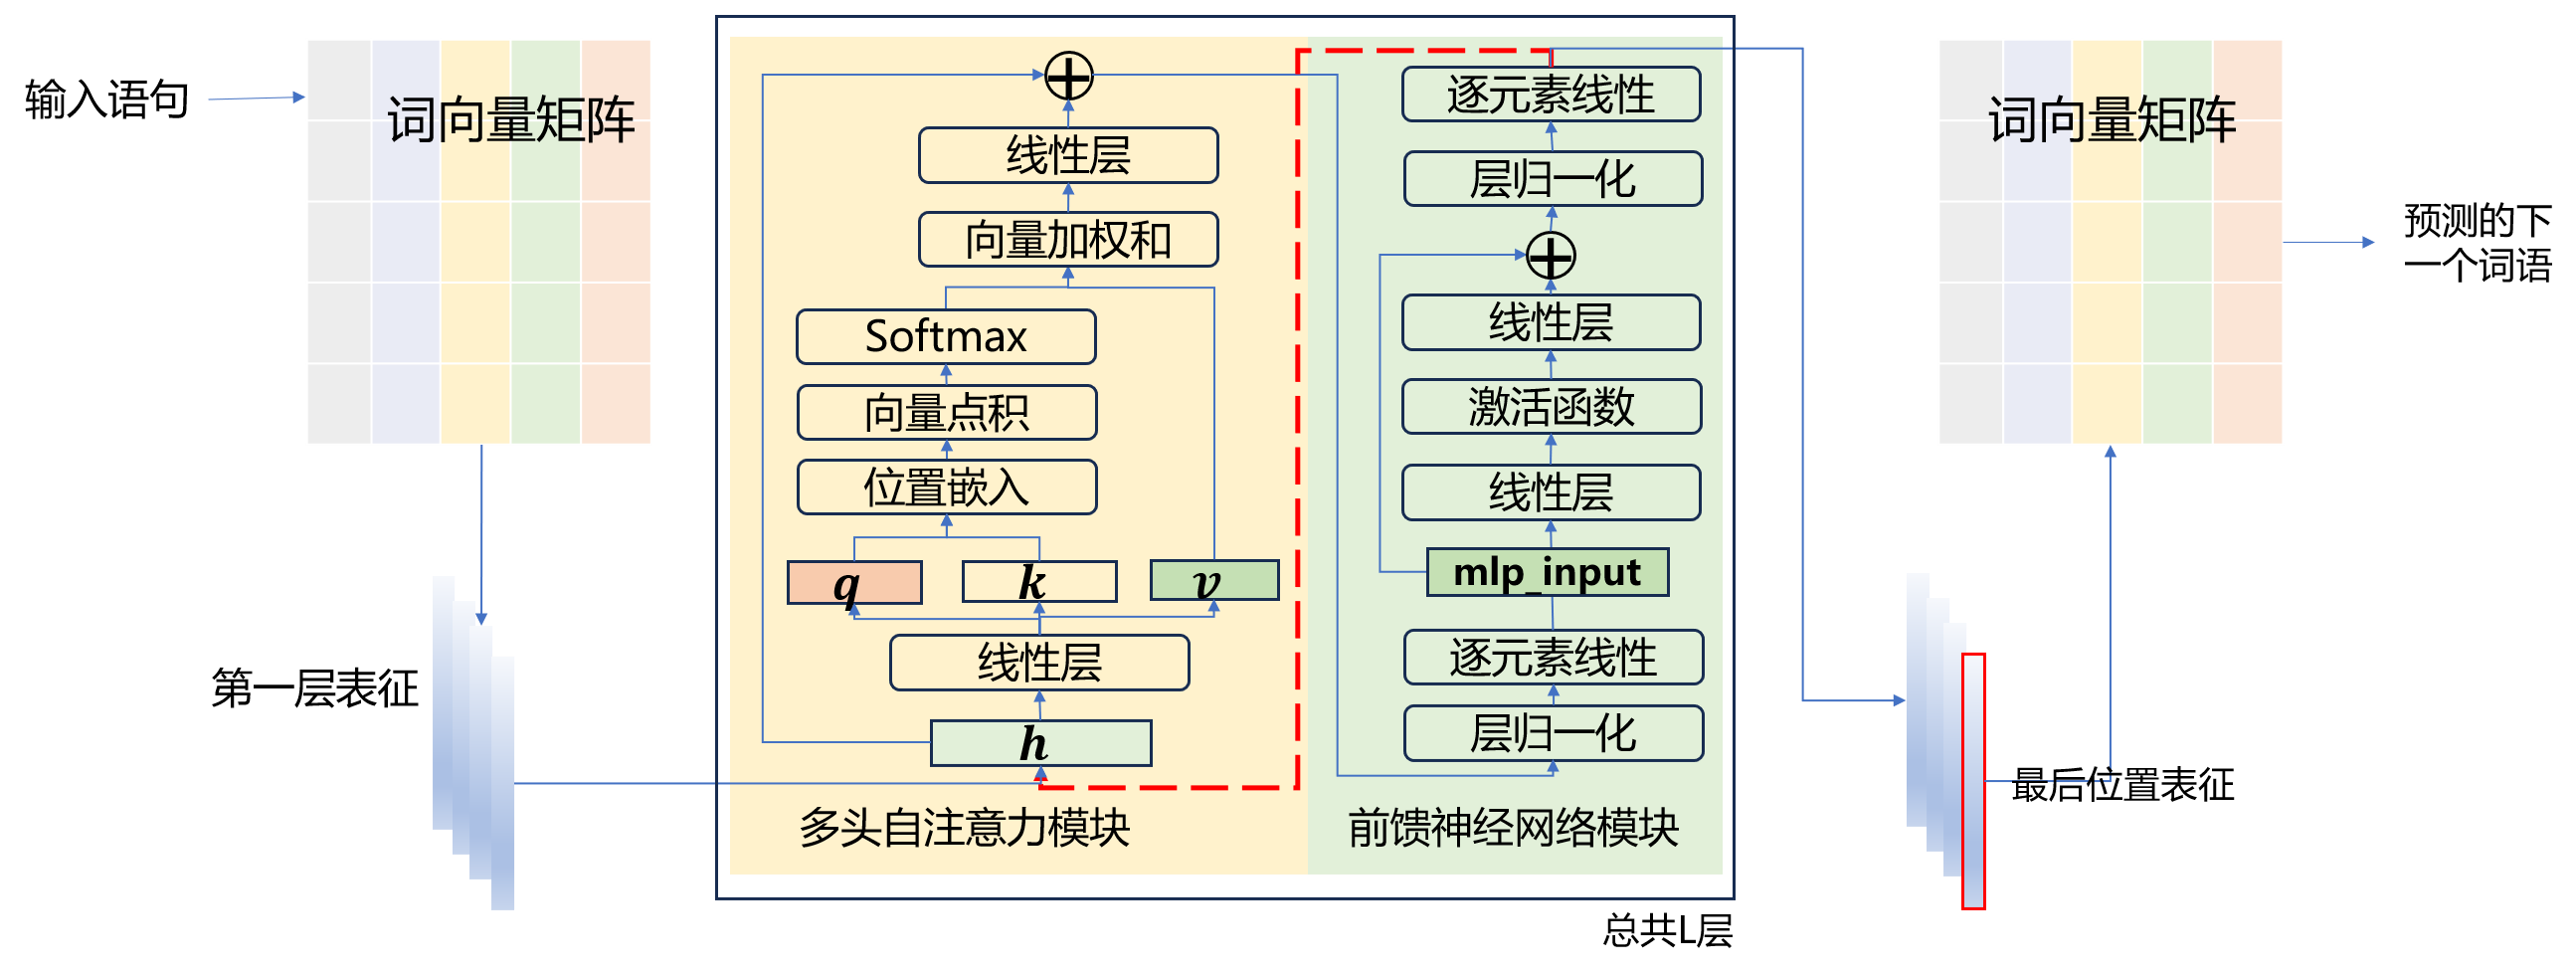
\includegraphics[width=\linewidth]{Z_Resources/perm-llm_llm-architecture.png}
    \caption{大语言模型结构示意图}
    \label{fig:perm-llm_llm-arch}
\end{figure}


\subsection{针对大模型拆分学习的攻击}
从上节的大模型结构描述中可以看出,大模型的隐层表征在每一层Transformer的变换中都保持着同样的大小,即$n \times d$($n$ 表示输入语句长度,$d$表示表征维度)。
%
因此从直观角度理解,大模型隐层表征包含了大量的输入信息。
且由于其隐层表征的尺寸随着层数增加保持不变,可以猜测即使是高层的隐层表征,依然包含着足够多的输入数据的信息。
%
已有研究提出可以通过训练逆向模型的方式从表征中恢复原始原本,无需知道模型的具体参数~\cite{morris2023embedding_almost}。
而本节则考虑攻击者已知模型参数的情况,更符合大模型的应用场景。


在拆分学习的大模型推断场景中,大模型被划分为一个底部模型$M_b$和一个顶部模型$M_h$。
%
我们假设模型拥有方最初拥有整个模型$(M_b, M_h)$,这也符合当前大模型训练是中心化的实际情况。
%
为了实现拆分学习的推断,模型拥有方将$M_b$发送给用户。
%
这种情况下,用户需要发送底部模型产生的表征$\bvec h = M_b(\bvec x)$给模型拥有方,其中$\bvec x$表示用户的输入文本对应的下标向量。

\subsubsection{表征逆向攻击}
当模型拥有方获取用户输入的表征后,就可以进行白盒攻击~\cite{hezecheng_2019_model_inversion_attack},通过如下的优化问题来猜测用户的输入:
\begin{equation}
    \label{eq:perm-llm_split-attack-0}
    \min \Vert M_b(\bvec x') - M_b(\bvec x)\Vert^2,
\end{equation}
其中$\bvec x'$是模型拥有方猜测的用户输入,$\bvec x$是用户的实际输入。
%
注意到直接对$\bvec x'$进行优化是较为困难的,因为其值域是离散的单词下标。
虽然可以转化成读热向量(One-Hot Vector),但是其依然具有离散的约束从而导致优化难以进行。
%
为此,模型拥有方可以首先优化初始表征$H'$,也就是词向量矩阵与(猜测的)用户输入对应的独热向量乘积:$H'_i = E\ \mathsf{onehot}(x'_i)$。
%
我们让$T_b$为底部模型除去词向量层(第一层)产生的模型,则我们可以把\autoref{eq:perm-llm_split-attack-0}改写为
\begin{equation}
    \label{eq:perm-llm_split-attack-1}
    \min \Vert T_b(H') - M_b(\bvec x)\Vert^2.
\end{equation}
由于此时优化变量$H'$属于连续变量,同时注意到$T_b$是模型拥有方已知的,因此我们可以直接用梯度下降等方法对\autoref{eq:perm-llm_split-attack-1}进行优化。
%
此时上述优化问题的未知数个数($H'$中的元素个数)与方程个数相等($M_b(\bvec x)$的元素个数),均为$nd$个元素,因为我们认为这个优化问题可能存在唯一的最优解,也就是$H' = H := (E\ \mathsf{onehot}(x_1), \cdots, E\ \mathsf{onehot}(x_n))$。
%
当得到猜测的表征$H'$之后,对于其中的第$i$行,使用余弦相似度计算出其最相似的词向量:
\begin{equation}
    \text{最相似单词下标} = \mathop{\text{argmax}}_i \dfrac{\bvec h'_i \cdot \bvec e_i}{\Vert \bvec h'_i \Vert\Vert \bvec e_i \Vert},
\end{equation}
其中$\bvec e_i$表示词向量矩阵的第$i$行。

综上所述,从大模型隐层表征恢复出用户输入文本的过程可以分为恢复第一层表征和从第一层表征恢复单词两步。
%
通过上述提出的两步方法,攻击者可以从隐层表征逆向推理出输入文本中每一个位置的单词,从而窃取用户的输入数据。
%

\subsubsection{可能的防御机制}
对数据加噪声是一种常用的隐私保护方法,并且在特定情况下可以达成差分隐私~\cite{dwork_2006_differential_privacy}。
%
因此,本节我们考虑在隐层表征中加入噪声进行防御的手段~\cite{morris2023embedding_almost}。
%
当用户算出底部模型产生的表征$H$后,对其进行扰动得到
\begin{equation}
    \tilde H_{ij} = H_{ij} + \lambda \cdot \epsilon, \quad \epsilon \sim \mathcal N(0, 1), 
\end{equation}
其中,$\lambda$表示噪声的大小。
%
越大的噪声一般可以实现越好的保护效果,但是也会产生更多的精度损失,损害模型性能。

\subsubsection{实验分析}
为了进一步测试上述攻击方案的可行性,我们在ChatGLM-6B模型~\cite{zeng_2022_glm130b}上进行了实验。
%
我们选用了Squad~\cite{2016_squad}和FindSum~\cite{2022_findsum}两个数据集进行实验,分别对应较短的文本和较长的文本。
%
对于每个实验,我们都对200个输入进行测试并且求其平均值。
%
攻击准确率的定义如下:
\begin{equation}
    \text{准确率} = \dfrac{1}{n} \sum_{i=1}^n \left( \dfrac{1}{l_i} \sum_{j=1}^{l_i} 1_{t'_{i,j} = t_{i,j}} \right),
\end{equation}
其中,$n = 200$表示总共的输入文本数,$l_i$表示第$i$个文本的长度,$t'_{i,j}$和$t_{i,j}$表示攻击得到的和实际的第$i$个文本的第$j$个单词。
%
由于ChatGLM-6B模型总共包含了28个Transformer层,我们设置拆分层分别为第10层和第20层。
%
我们使用梯度下降算法迭代优化\autoref{eq:perm-llm_split-attack-1}直到$H'$和$H$的余弦相似度达到0.98或迭代步数达到1000步为止。
%
我们使用半精度浮点数进行运算。

\begin{figure}[h!]
    \centering
    \begin{subfigure}{0.48\linewidth}
    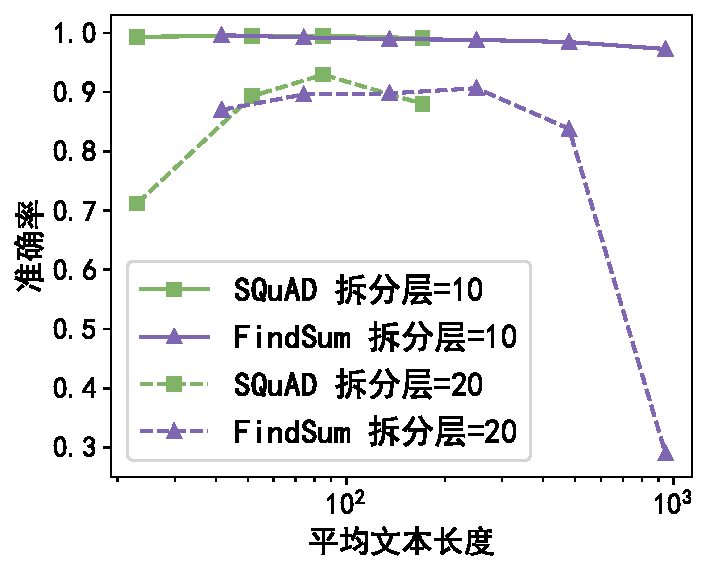
\includegraphics[width=\linewidth]{Z_Resources/perm-llm_seqlen-acc.pdf}
    \caption{攻击准确率}
    \end{subfigure}
    %
    \begin{subfigure}{0.48\linewidth}    
    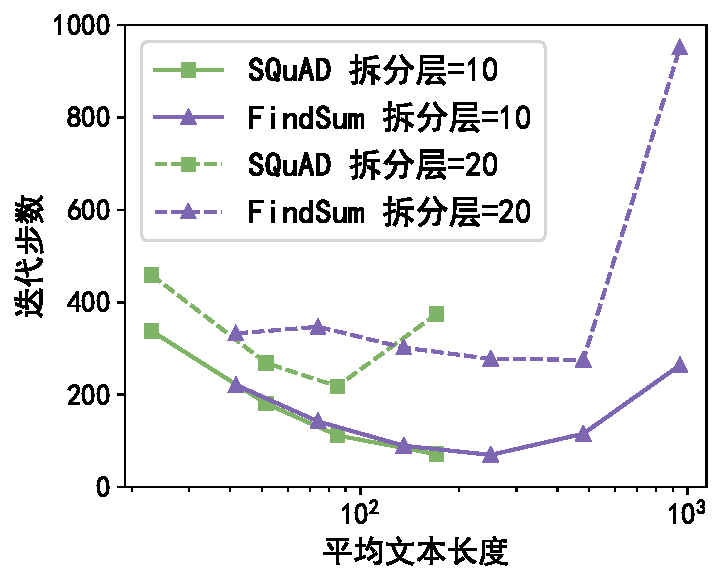
\includegraphics[width=\linewidth]{Z_Resources/perm-llm_seqlen-steps.pdf}
    \caption{攻击所需迭代步数}    
    \end{subfigure}
    \caption{攻击效果与文本长度的关系}
    \label{fig:perm-llm:attack-seqlen}
\end{figure}


\begin{figure}[h!]
    \centering
    \begin{subfigure}{0.48\linewidth}
    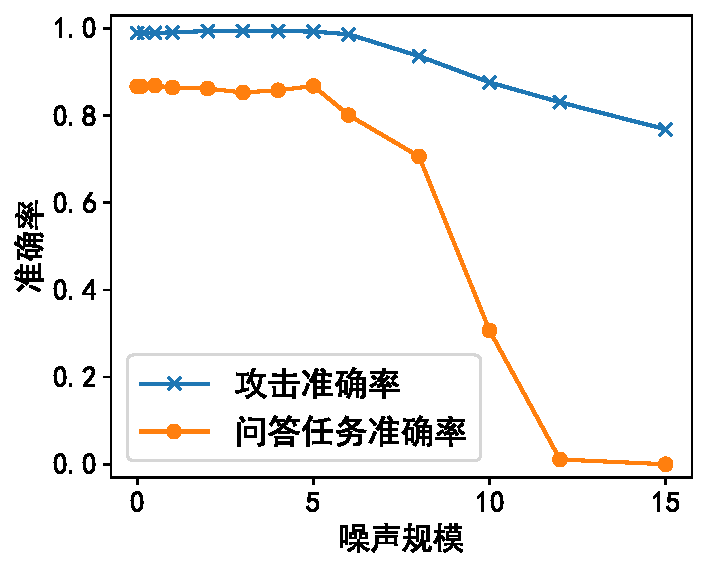
\includegraphics[width=\linewidth]{Z_Resources/perm-llm_squad-noise-layer10.pdf}
    \caption{拆分层=10}
    \end{subfigure}
    %
    \begin{subfigure}{0.48\linewidth}    
    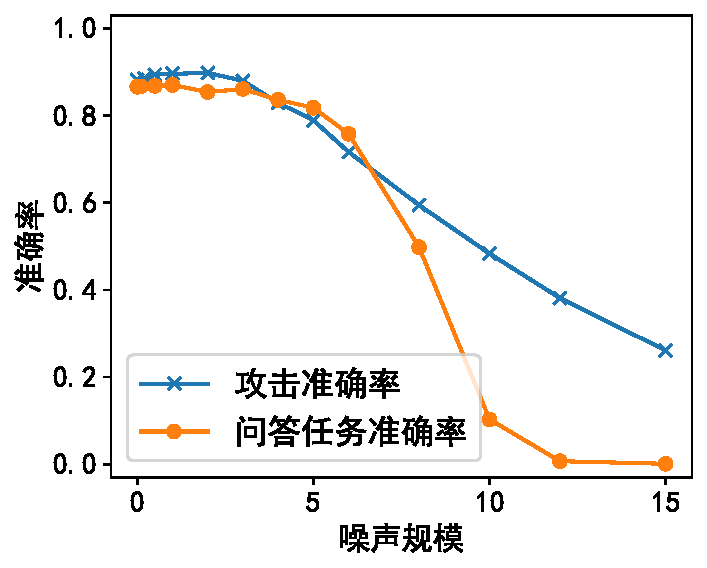
\includegraphics[width=\linewidth]{Z_Resources/perm-llm_squad-noise-layer20.pdf}
    \caption{拆分层=20}    
    \end{subfigure}
    \caption{攻击效果与噪声大小的关系}
    \label{fig:perm-llm:attack-noise}
\end{figure}

%
我们首先测试了对于不同输入语句长度的逆向攻击效果,测量了窃取用户输入文本的准确率以及迭代所用次,并呈现在\autoref{fig:perm-llm:attack-seqlen}中。
%
从图中可以看出,在拆分层为第10层时,无论文本长度多长,攻击都能达到接近100\%的准确率;而拆分层在20层时,攻击准确率略有下降,大概为90\%左右。
同时我们注意到,文本长度特别长(1000左右)或特别短(个位数)时,攻击效果也会下降。
%
特别是文本长度达到1000时,攻击效果下降明显,但是此时迭代步数也达到了我们预设的最高值,因此可能在更多的迭代步数下会达到更高的效果。
%
此外,提高浮点运算的精度(比如从16位半精度提升到32位单精度)也可能会提升攻击效果。


我们也在Squad数据集上测试了噪声规模$\lambda$的大小对攻击效果以及原始任务效果的影响。
其中原始任务的准确率指的是问答任务的准确率,按照大模型返回的字符串中是否包含参考答案的字符串来计算,若包含则为回答正确,反之则为回答错误。
%
我们将结果汇报在\autoref{fig:perm-llm:attack-noise}中。
%
可以看到,随着噪声规模的增加,攻击准确率呈现出下降趋势。
然而原始的问答任务准确率也同步开始下降,并且下降速度更快。
%
在拆分层为第10层时,当问答任务的准确率已经变成0之后,攻击准确率依然有80\%以上。
在拆分层为第20层时,两者的下降幅度更加接近,但是问答任务准确率依然在$\lambda \ge 5$后下降的更快并且更快归零。
%



上述的实验分析表明,攻击者可以通过大模型拆分层的表征,有效地以很高精度还原出用户的原始输入。
%
对拆分层表征添加噪声的防御手段并不能有效地避免此种攻击。
%
这说明拆分学习不适用于大模型隐私推断的场景。

\section{PermLLM框架}
经过前文的梳理和分析,我们可以看到拆分学习应用于大模型的隐私推断存在严重的隐私泄漏问题,与此同时,密码学方法则存在着严重的计算通讯开销问题。
%
我们注意到,密码学在进行大模型隐私推断时,其主要的开销也在于非线性激活函数GeLU上。
由于GeLU的非线性较强,各种密码学方案往往采用高阶多项式对其进行拟合,从而带来了严重的计算开销。
%
现有研究的分析表明,GeLU、层归一化等的通讯开销甚至可以达到线性计算(矩阵乘法等)的一百多倍。
%
因此,优化基于密码学的大模型隐私推断的关键在于优化非线性函数。
%
%

而上一章提出的基于秘密分享和随机排列的安全神经网络框架正是对神经网络的非线性激活函数进行优化,极大提高了神经网络隐私推断和训练的效率,同时尽可能地维持了安全性。
%
在此基础上,本章我们对此针对大模型进行进一步优化,提出融合密码学方法和随机排列的基础上,实现高效安全的大模型隐私推断框架PermLLM。
%
PermLLM框架面向的场景为两方推断的场景,且存在一个辅助第三方用于离线计算。
%
$P_0$为模型拥有方(如OpenAI),其拥有模型的所有参数信息。
%
$P_1$为用户,其目标是获取大模型的关于自身的文本输入的回复。
%
$P_2$为辅助第三方,其参与离线计算阶段,用于生成安全乘法和安全排列的预计算值。
%
我们采用了半可信的安全性设定,同\autoref{}一致。


我们将大语言模型的计算分为三个部分:线性部分、非线性部分和下标选择阶段。
其中线性阶段包含了线性层、注意力分数计算、层归一化后的逐元素线性映射等;
非线性阶段包含了GeLU激活函数、注意力分数的Softmax计算、层归一化的计算等;
而下标选择阶段则是根据预测的分数安全地产生预测词语的下标的阶段。
%
对于线性阶段,我们通过改进的秘密分享协议进行高效计算;
对于非线性阶段,我们采用基于安全随机排列协议的逐元素计算协议进行计算;
对于下标选择阶段,我们基于随机排列和同态加密设计了安全的下标选择协议,不仅支持常用的选取最大分数的词语,也支持按照概率采样等复杂的下标选择策略。
%


\subsection{隐私推断的三个阶段}
许多基于秘密分享技术的隐私保护机器学习框架会按照两个阶段运行,分别是离线(Offline)阶段和在线(Online)阶段。
%
考虑$P_0$和$P_1$要安全地计算$f(X)$的情况,其中$X$被秘密分享在两方之间,而$f$则是一个固定的函数。
%
在离线阶段,$X$还未出现,$P_0$和$P_1$并不需要知道$X$的具体值。
%
但是其可以对未来的$f(X)$进行一些准备工作,比如生成Beaver三元组来辅助安全乘法计算。
%
在在线阶段,$P_0$和$P_1$得到了$X$的具体值,再进行后续的工作。
%t
通过这种方法,参与方可以在还未进行具体的隐私计算任务时提前准备,从而可以减少具体输入出现后的安全计算的开销。

%
而在PermLLM中,我们采用类似的思想,将隐私推断分为三个阶段,分别是初始化阶段、离线阶段、在线阶段。
%
其中初始化阶段和对应的大模型权重有关,在大模型权重不改变的情况下,初始化阶段仅需执行一次。
%
离线阶段和在线阶段则和一般隐私保护机器学习框架中的定义相同。
每一次离线阶段会产生一些预计算值供在线阶段使用,而每一次在线阶段都会消耗一次离线阶段产生的预计算值。
%
比如,一个可能的运行序列可以是“初始化-离线-在线-离线-在线”,
也可以是“初始化-离线-离线-在线-在线”。
但是“初始化-离线-在线-在线-离线”是一个不合法的顺序,因为第二个在线阶段时已经没有预训练的值供其使用。

\subsection{优化的秘密分享乘法}


\subsubsection{针对线性层的秘密分享乘法}
我们首先考虑大预言模型中的线性层。
%
线性层的计算可以表示为$W \bvec x + \bvec b$,其中$W \in \mathbb R^{d\times d}$是一个大矩阵,表示权重;$\bvec x \in \mathbb R^{d}$则是输入文本相关的隐层表征。
%
在秘密分享中,共有两次通讯,分别是离线时$P_2$分发Beaver三元组($U\bvec v = \bvec w$)给$P_0$和$P_1$,和在线时$P_0$和$P_1$恢复出$W - U$和$\bvec x - \bvec v$。
%
我们注意到,由于大模型推断过程中权重$W$是固定不变的,我们可以产生一次Beaver三元组中的$U$,同时$W - U$也只需恢复一次。
因此我们可以把这些计算安排到初始化阶段进行。
%
而输入相关的$\bvec x$则会每次变化,因此三元组中的$\bvec v$和对应的$\bvec w=U\bvec v$会被每一次在线运算阶段消耗,需要在每次离线阶段重新生成。
%
因为$W$的大小是$\bvec x$的$d$倍(在大语言模型中$d > 10^3$),因此将有关$W$的计算提前到初始化阶段单次计算,可以极大地减少在线阶段和离线阶段的通讯开销。


我们在\autoref{alg:perm-llm:secure_mul_fixed}中具体描述上述算法。
同时,在\autoref{fig:perm-llm:ssmul}中,我们也对比了原始的秘密分享乘法和优化的$X$固定的秘密分享乘法。
%
利用$X$是$P_0$已知的特性,我们可以把$P_0$计算的$(X-U)(Y-V) + \langle U \rangle_0(Y-V)$,以及$P_1$计算的$\langle U \rangle_1(Y-V)$合并,
变成仅需$P_0$计算$X(Y-V)$。
%
此时$P_1$无需知道$Y-V$,只需将自身的$\langle Y \rangle_1 - \langle V \rangle_1$发送给$P_0$即可。
因此我们进一步将在线阶段的通讯次数从2轮减少到1轮。
%


\begin{algorithm}[h!]
    \caption{安全常数乘法\textsf{SecureMul}$_F(X, Y)$}
    \label{alg:perm-llm:secure_mul_fixed}
    \begin{algorithmic}[1]
    \Require $P_0$ 持有常数 $X$. 秘密分享的输入 $\langle Y \rangle$
    
    \Ensure 秘密分享的乘积 $\langle Z \rangle = \langle XY \rangle$
    
    \item[\underline{初始化阶段:}]
    %
    \State $P_2$ 产生随机的 $U$ (和 $X$ 形状相同) 并发送给 $P_0$
    %
    \State $P_0$ 发送 $X - U$ 给 $P_1$
    
    \item[\underline{离线阶段:}]
    \State $P_2$ 产生随机的 $V$ (和$Y$ 形状相同), 并且分享 $V, W \gets UV$ 给 $P_0$ 和 $P_1$
    
    \item[\underline{在线阶段:}]
    \State $P_1$ 发送 $\langle Y \rangle_1 - \langle V \rangle_1$ 给 $P_1$,$P_1$ 恢复 $X - U$
    %
    \State $P_0$ 计算 $\langle Z \rangle_0 \gets X(Y-V) + (X-U)\langle V \rangle_0 + \langle W \rangle_0$
    %
    \State $P_1$ 计算 $\langle Z \rangle_1 \gets (X-U) \langle V \rangle_1 + \langle W \rangle_1$
    \end{algorithmic}
\end{algorithm}


\begin{figure}[h!]
    \centering
    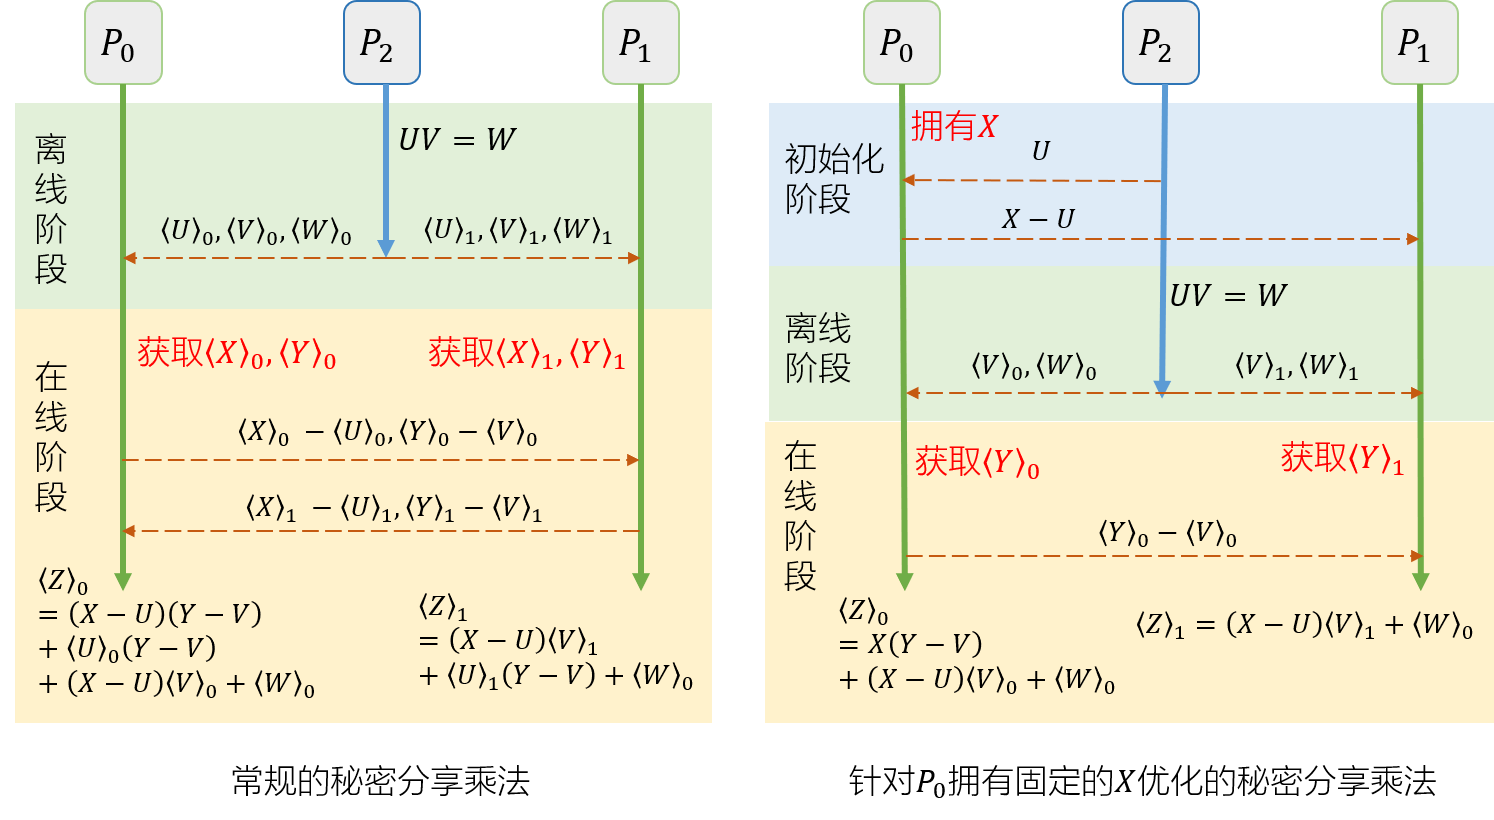
\includegraphics[width=\linewidth]{Z_Resources/perm-llm_ssmul.png}    
    \caption{优化的秘密分享乘法与原始秘密分享乘法的对比}
    \label{fig:perm-llm:ssmul}
\end{figure}


\subsubsection{针对注意力的秘密分享乘法}
在计算注意力分数时,我们需要将当前的查询向量 $\bvec q_i$ 与多个键向量 $\bvec k_1, \cdots, k_n$ 求内积,且注意到在单次文本生成任务中,每轮都会有一个新的键向量加入。
%
如果把键向量构成的矩阵当作$X$,我们可以发现情况与线性层有所类似。
乘数$X$虽然不是固定的,但是其每一轮只会加入一个新的向量,而其余部分保持不变。
%
因此,我们可以借用针对线性层优化的安全秘密分享乘法中的思想,在每一轮在线阶段的运算中,只考虑 $X$ 新增加的部分(此处记作$X'$)恢复出 $X' - U'$,从而更新原有的 $X - U$上。
%
\section{安全性分析}
本节我们对PermLLM进行的安全性进行分析,表明其泄漏的隐私是忽略不计的。
%
我们分别对随机排列和浮点数秘密分享的安全性进行分析。


\subsection{随机排列}
在PermLLM中,随机排列用于注意力分数的Softmax计算、激活函数的计算,以及最终的单词分数解码中。
%
首先考虑注意力分数,假设有$h$个注意力头,键值向量个数为$n$,则总共有$h!(n!)^h$种随机排列的方式。
即使$n=1$,也有$h!$种排列。
在大语言模型中,$h \ge 32$,因此$h! > 2^{117}$,因此猜测出实际排列的概率可以忽略不计。
%
而对于激活函数,则排列元素个数为隐层大小,超过$1000$;对于单词分数,则其元素个数为词汇表大小,超过$10$万。
因此这些情况恢复出原始排列的可能性更加接近0。
%
除此之外,我们在第\ref{chap:ss-perm}章中对随机排列的值和原始值的相关性进行了详尽分析,表明随机排列后的值和原始值在距离相关性~\cite{szekely2007dcor}的意义下相关程度非常低,也就是说其暴露的原始值的隐私信息也是极小的。


\textbf{暴力搜索攻击}:
一种针对随机排列的攻击是暴力搜索(Brute-Force Search)攻击。
对于随机排列后的结果$\bvec y' = \pi[f(\bvec x)]$,攻击者可以选取所有可能的输入$\bvec x' \in X$,并检查$f(\bvec x')$是否与$f(\bvec x)$的元素相同。
这是因为随机排列只会改变向量中元素的顺序,但是还是会保留原始的元素集合。
在不考虑计算资源的情况下,若函数的输入$\bvec x$的取值是有限的,则攻击者理论上可以通过暴力搜索攻击从随机排列的输出推出(可能的)原始的输入。
%
由于大语言模型输入是离散的,因此也存在暴力搜索攻击的风险。
但是PermLLM巧妙地回避了此种攻击。
%
在PermLLM中,只有$P_1$(用户)才能获得随机排列后的明文,而$P_1$本身也是离散输入的拥有方,因此不存在暴力破解的可能性。

\subsection{浮点数秘密分享}
在浮点数秘密分享中,任何一个数$x$的分享值满足
\begin{equation}
\begin{cases}
    \langle x \rangle_0 = D, & \text{其中} \mathbb E[D^2] = \lambda^2\mathbb E[x^2], \\
    \langle x \rangle_1 = x - D.
\end{cases}
\end{equation}
此处为了方便,我们假设$\mathbb Ex = \mathbb ED = 0$。
%
可见$\langle x \rangle_0$与$x$无关,而$\langle x \rangle_1$是$x$加入一个规模是其$\lambda$倍的巨大噪声的结果。
%
同时我们也注意到,在执行秘密分享的乘法时,$x - u$会暴露给双方,此时$\mathbb E[u^2] = 2\lambda^2 \mathbb E[x^2]$。
%
对于秘密分享乘法的结果$z = xy$,在产生Beaver三元组的时候我们已经选取了$\mathbb E \langle w \rangle_0 = \lambda^2 \mathbb E[z^2]$,因此$\langle z \rangle_0$ 与 $z$无关,而$\langle z \rangle_0$ 是$z$加上一个规模为其$\lambda$倍的噪声。
%
综上所述可以得出,对于任何一个值$x$,采用浮点数秘密分享时,各方获取到的数据$x'$只有两种情况:
\begin{enumerate}[label=(\arabic*)]
    \item $x'$与$x$无关;
    \item $x' = x + D$,$D$为与$x$无关的随机变量且$\mathbb E[D^2] = \lambda^2 \mathbb E[x^2]$。
\end{enumerate}
%
当$\lambda$很大时,$x'$暴露的关于$x$的信息暴露可以忽略不计。
%
但是如果使用同样的输入变量进行多次浮点秘密分享计算,则攻击者可以通过多次平均的方式来获取原始的值。
%
假设$x$是原始值,攻击者获取的加噪值为$x_1, \cdots, x_n$,则有:
\begin{equation}
\begin{split}
    \mathbb E\left[\left(\dfrac{x_1 + \cdots + x_n}{n} - x \right)^2 \right] = 
    \mathbb E\left[\dfrac{(x_1 - x)^2 + \cdots + (x_n - x)^2}{n^2} \right] =
    \dfrac{\lambda^2}{n}.
\end{split}
\end{equation}
%
若选取$\lambda = 100$,则攻击者(如$P_1$)采用同样的输入进行10万次隐私推断,并对上述秘密分享值进行平均,可以将误差缩小到原始数据规模的$1/10$水平:
$\sqrt{\mathbb E[(\bar x - x)^2]} = {\mathbb E[x^2]}/{10}$。
%
此时$P_1$可能根据这些估计的秘密分享值,也就是隐私推断中的中间结果,反推出模型权重,从而实现窃取模型的目的。
%
因此,采用浮点数秘密分享时,必须要采取额外的手段来防止上述攻击的产生。可能的方案有:采用第三方对$P_1$的输入文本进行验证;$P_0$设计一定的手段检测恶意行为;以及当隐私推断达到一定次数后,对模型进行恒等变换来改变权重值~\cite{xuhengyuan_2024_permutation_transformer},再重新执行初始化阶段分享权重等。
%



\section{实验分析}
为了验证所提出的PermLLM方法,我们在不同的设定下进行了实验,包括了不同的网络环境以及不同的Transformer模型大小。
%
我们的当前最新的基于密码学的大语言模型或Transformer模型隐私推断框架进行了对比,包括MPCFormer~\cite{li2022mpcformer}和Puma~\cite{dong2023puma}。
%
这些实验在搭载4张NVIDIA RTX 3090 (24G)显卡的服务器上进行。
%
此外,我们使用PermLLM框架实现了ChatGLM-6B模型~\cite{zeng_2022_glm130b},并在搭载有3台NVIDIA L20 (48G)的显卡的服务器上进行了实验。
%

我们考察了以下的网络环境:
\begin{itemize}
    \item LAN (Local Area Network):此时我们经由本机IP地址(127.0.0.1/localhost)进行通信,而未进行实际的网络通信。
    \item WAN1:往返时延为10ms,相当于400千米距离的网络时延,如东京到大阪;网络带宽为1Gbps,对应商用水平的网络连接。
    \item WAN2:往返时延为20ms,相当于1000千米距离的网络时延,如柏林到伦敦;网络带宽为100Mbps,对应家用网络。
\end{itemize}


\subsection{基准测试}
我们首先对非线性函数计算和单层的Transformer推断进行了基准测试,并且测量了通信量、通信轮数和总的执行时间。
我们将非线性函数的结果汇报在\autoref{tab:perm-llm:nonlinear}中,将单层Transformer结果汇报在\autoref{tab:perm-llm:layer}中。
%

%
\begin{table}[h!]
    \small
    \caption{非线性函数的基准测试(注:LN表示层归一化,any表示任意非线性函数)}
    \label{tab:perm-llm:nonlinear}
    \begin{tabular}{@{}cccrrrrr@{}}
    \toprule
    $f$ & $n$ & 方法 & 通信(Mb) & 轮数 & LAN & 1Gbps/10ms & 100Mbps/20ms \\ \midrule
    \multirow{6}{*}{\parbox[t]{2mm}{\multirow{3}{*}{\rotatebox[origin=c]{90}{Argmax}}}} & \multirow{3}{*}{1K} & MPCFormer & 1.24 & 101 & 0.09 ± 0.01 & 2.11 ± 0.00 & 4.12 ± 0.01 \\ \cmidrule(l){3-8} 
     &  & Puma & $\approx$0.80 & $\approx$1700 & 0.15 ± 0.03 & 3.29 ± 0.03 & 6.33 ± 0.05 \\ \cmidrule(l){3-8} 
     &  & \textbf{PermLLM} & \textbf{0.26} & \textbf{4} & \textbf{0.03 ± 0.00} & \textbf{0.05 ± 0.00} & \textbf{0.06 ± 0.01} \\ \cmidrule(l){2-8} 
     & \multirow{3}{*}{100K} & MPCFormer & 110.9 & 153 & 0.78 ± 0.04 & 4.04 ± 1.41 & 10.74 ± 0.50 \\ \cmidrule(l){3-8} 
     &  & Puma & $\approx$80 & $\approx$2500 & 1.17 ± 1.13 & 6.23 ± 0.08 & 12.88 ± 0.06 \\ \cmidrule(l){3-8} 
     &  & \textbf{PermLLM} & \textbf{4.02} & \textbf{4} & \textbf{0.12 ± 0.01} & \textbf{0.17 ± 0.01} & \textbf{0.2 ± 0.00} \\ \midrule
    \multirow{6}{*}{\parbox[t]{2mm}{\multirow{3}{*}{\rotatebox[origin=c]{90}{Element-wise}}}} & \multirow{3}{*}{1K} & Puma: GeLU & $\approx$1.7 & $\approx$200 & 0.04 ± 0.02 & 0.38 ± 0.02 & 0.71 ± 0.01 \\ \cmidrule(l){3-8} 
     &  & Puma: LN & $\approx$0.20 & $\approx$200 & 0.02 ± 0.00 & 0.35 ± 0.01 & 0.67 ± 0.01 \\ \cmidrule(l){3-8} 
     &  & \textbf{PermLLM: any} & \textbf{0.01} & \textbf{3} & \textbf{0.00 ± 0.00} & \textbf{0.02 ± 0.00} & \textbf{0.04 ± 0.01} \\ \cmidrule(l){2-8} 
     & \multirow{3}{*}{\begin{tabular}[c]{@{}c@{}}100K\\100$\times$1K\end{tabular}} & Puma: GeLU & $\approx$170 & $\approx$200 & 1.32 ± 0.11 & 1.69 ± 0.23 & 12.37 ± 0.08 \\ \cmidrule(l){3-8} 
     &  & Puma: LN & $\approx$20 & $\approx$200 & 0.13 ± 0.03 & 0.15 ± 0.02 & 0.83 ± 0.03 \\ \cmidrule(l){3-8} 
     &  & \textbf{PermLLM: any} & \textbf{1.15} & \textbf{3} & \textbf{0.01 ± 0.00} & \textbf{0.03 ± 0.01} & \textbf{0.05 ± 0.00} \\ \bottomrule
    \end{tabular}
\end{table}


\begin{table}[h]
\small
\centering
\caption{单层Transformer的基准测试}
\label{tab:perm-llm:layer}
\begin{tabular}{@{}ccrrrrr@{}}
\toprule
模型大小 & 方法           & 通信(Mb)   & 轮数        & LAN                   & 1Gbps/10ms            & 100Mbps/20ms         \\ \midrule
\multirow{3}{*}{\begin{tabular}[c]{@{}c@{}}Large\\ ($d=4096$)\end{tabular}} & MPCFormer & 3073.79 & 53 & 1.37 ± 0.01 & 26.15 ± 0.35 & 259.65 ± 0.36 \\ \cmidrule(l){2-7} 
            & Puma        & $\approx$33   & $\approx$1500 & 8.82 ± 0.09           & 11.45 ± 0.42         & 14.40 ± 0.65         \\ \cmidrule(l){2-7} 
            & \textbf{PermLLM} & \textbf{0.49} & \textbf{20}   & \textbf{0.04 ± 0.01}  & \textbf{0.12 ± 0.01} & \textbf{0.24 ± 0.00} \\ \midrule
\multirow{3}{*}{\begin{tabular}[c]{@{}c@{}}Small\\ ($d=768$)\end{tabular}}  & MPCFormer & 108.32  & 53 & 1.29 ± 0.19 & 1.71 ± 0.01  & 10.29 ± 0.20  \\ \cmidrule(l){2-7} 
            & Puma         & $\approx$6    & $\approx$1000 & 0.46 ± 0.03           & 2.24 ± 0.03          & 3.97 ± 0.04          \\ \cmidrule(l){2-7} 
            & \textbf{PermLLM} & \textbf{0.1}  & \textbf{20}   & \textbf{0.034 ± 0.00} & \textbf{0.15 ± 0.01} & \textbf{0.23 ± 0.02} \\ \bottomrule
\end{tabular}
\end{table}

可以看到,对于非线性运算而言,在任意输出规模或网络环境下,PermLLM框架都达到了最高的效率,其通信轮数、通信量以及时间消耗都显著低于对比算法。
%
不同于对比算法需要针对特定的非线性函数设计安全计算协议,PermLLM框架通过随机排列的方法,任何逐元素非线性函数都能在3轮通信中完成计算。
%
同时,其通信量也只是明文大小的4倍。
%
对于Argmax函数,我们使用的基于同态加密的安全下标抽取算法,只需要进行数十次同态乘法和同态加法,即可完成计算,其速度也领先于对比算法。

同样地,对于单层Transformer推断,PermLLM也达到了最大的效率。
%
且对于更大的Transformer,PermLLM的优势更大,说明了其在大语言模型中会具有更大的优势。
当Transformer的维度从768提升到4096后,其优势从一个数量级提升至两个数量级。
%
我们也注意到,在MPCFormer~\cite{li2022mpcformer}中,其采用Crypten框架~\cite{knott2021crypten}默认的算子进行秘密分享乘法,没有考虑到大语言模型的权重固定情况。
%
每一次秘密分享乘法时,都会对权重产生新的Beaver三元组并分发给$P_0$和$P_1$,以及恢复遮罩过的权重($X - U$),带来了巨大的额外性能损耗。


\subsection{ChatGLM-6B测试}
我们使用PermLLM框架实现了ChatGLM-6B模型~\cite{zeng_2022_glm130b},并且在两个WAN (Wide Area Network) 网络环境下进行了实验。
%
我们选择了6,15,37和62长度的输入文本,测量了每生成一个单词所需的时间和流量,绘制在\autoref{fig:perm-llm:chatglm}中。
%
可以看到,在WAN2(20ms/100Mbps)环境下,每个单词生成的时间大概在7秒左右;而在更快的WAN1(10ms/1Gbps)下,单词生成的时间仅需3秒左右。
%
注意到第一个单词产生的时间较长,这是因为在第一个单词生成时,要把整个输入文本放入模型进行推断;但是因为我们采用了键值缓存技术,之后只需要放入新生成的文本即可。
%
这个实验证明了PermLLM可以在普通的网络环境下把大模型隐私推断的时间提升到秒级别,相比于现有的密码学方案提升了两个数量级以上,从而使其具备一定的实用性。
%

\begin{figure}[htbp]
    \centering
    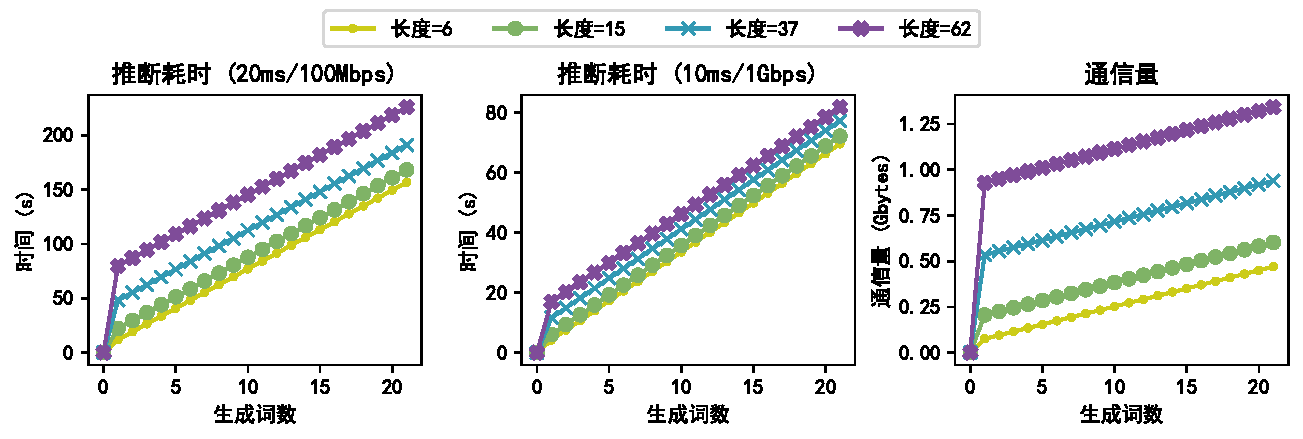
\includegraphics[width=\linewidth]{Z_Resources/perm-llm_ChatGLM.pdf}
    \caption{ChatGLM-6B实验结果}
    \label{fig:perm-llm:chatglm}
\end{figure}


此外,实验也观察到PermLLM框架几乎不会有准确率的损失。
%
这是因为浮点秘密分享的情况下,误差来源仅为秘密分享计算中的浮点计算舍入误差(Rounding Error)。
%
即使将其转化为整数计算,只需要设置精度位,同样可以实现几乎无误差的隐私推断。
%
对比之下,基于密码学的方法由于采用了多项式拟合GeLU等技术,会带来除去舍入误差之外的更大误差。
\section{本章小结}
本章我们研究了大语言模型的隐私推断问题,提出了拆分学习在此问题上的不可行性。
%
针对密码学方法的大语言模型隐私推断中非线性激活函数开销大的问题,我们基于第\ref{chap:ss-perm}章提出的隐私保护神经网络框架进行改进,对秘密分享乘法和非线性函数计算协议进行进一步优化,结合同态加密技术,实现了高效的大模型隐私推断框架PermLLM。
%
我们利用PermLLM框架实现了ChatGLM-6B模型,在现实的网络环境下实现了秒级别的隐私推断速度,为大语言模型隐私推断的实用打下了基础。